
%(BEGIN_QUESTION)
% Copyright 2011, Tony R. Kuphaldt, released under the Creative Commons Attribution License (v 1.0)
% This means you may do almost anything with this work of mine, so long as you give me proper credit

In this automotive fuel level sensing circuit, a current mirror is supposed to maintain a constant current (about 25 to 26 mA) through the fuel level sensor, which is nothing more than a variable resistance (rheostat) that changes with fuel level.  The voltage dropped across this sensor resistance is then sent to a fuel gauge: a voltmeter with the scale calibrated in gallons of fuel level:

$$\includegraphics[width=15.5cm]{i03286x01.eps}$$

There is a problem in this circuit, though.  The fuel gauge reads full even when you know the fuel tank is completely empty.  You take two DC voltage measurements to begin your troubleshooting: +11.5 volts between TP2 and ground, and 11.7 volts between TP3 and ground.

From this information, identify two possible faults (either one of which could account for the problem and all measured values in this circuit), and also identify two circuit elements that could not possibly be to blame (i.e. two things that you know {\it must} be functioning properly, no matter what else may be faulted).  The circuit elements you identify as either possibly faulted or properly functioning can be wires, traces, and connections as well as components.  Be as specific as you can in your answers, identifying both the circuit element and the type of fault.

\medskip
\goodbreak
\item{} Circuit elements that are possibly faulted
\item{1.}
\item{2.} 
\end{itemize}

\medskip
\goodbreak
\item{} Circuit elements that must be functioning properly
\item{1.} 
\item{2.} 
\end{itemize}

\vfil 

\underbar{file i03286}
\eject
%(END_QUESTION)





%(BEGIN_ANSWER)

This is a graded question -- no answers or hints given!

%(END_ANSWER)





%(BEGIN_NOTES)

A good problem-solving strategy to apply here is calculating the expected voltages in a healthy circuit.  The voltage value of 11.5 volts at TP2 seems reasonable, because the ``crippled'' $Q_1$ acting as a diode should drop somewhere in the neighborhood of 0.5 to 0.7 volts, making the voltage between TP2 and ground that much less than the supply voltage of 12 volts.  The voltage at TP3, however, is not what we would expect to see in a healthy circuit.

\vskip 10pt

The voltage at test point TP3 should range between 0.13 and 6.8 volts (the proper current multiplied by the sensor's resistance values at each extreme).  The fact that we're reading much more than this at TP3 suggests either we are pushing too much current through the fuel level sensor resistance, or the resistance of that sensor is too great.

\begin{itemize}
\item{} Circuit elements that are possibly faulted
\item{1.} Transistor $Q_2$ failed shorted (partially, not completely)
\item{2.} Fuel sensor failed open
\end{itemize}

\begin{itemize}
\item{} Circuit elements that must be functioning properly
\item{1.} Ignition switch
\item{2.} Battery
\end{itemize}

%INDEX% Troubleshooting review: electric circuits

%(END_NOTES)


